\section{Sliceplorer}

When developing Sliceplorer, I first identified design requirements with
respect to tasks that a user would perform when analyzing multi-dimensional
scalar functions. I continuously evaluated how the technique fits with these
requirements and iteratively adapted it to encompass as many tasks as possible.
A static slice view itself does not address many of the tasks required so I
use interaction methods to address these and create a comprehensive technique.  

\subsection{Design requirements}

When analyzing a function visually, there are a number of features that the
user wants to see.

\textbf{R-peaks}: The most obvious feature
is identifying peaks and valleys. This is primarily done to find the
global optimum of a function. 

\textbf{R-robust}: The relative height
around each optima is important to detecting the robustness of that optimum. In
some cases one may prefer a local optimum over a global one if it is more stable.
This is very common in
simulations of manufacturing processes where variations in manufacturing tolerances
should not affect the performance of a part too much~\cite{Berger:2011}.  

\textbf{R-bowl}: Similarly, we may be
interested in how ``bowl''-shaped the area around an optimum is. The goal is
similar to robust optimization but rather than looking for ``flat'' areas of
the function we are looking for areas with smooth gradients. The amount of this
smoothness is important for correctly parameterizing optimization
algorithms~\cite{Back:1996}. An incorrect parameterization can either cause them to
get ``stuck'' at some local minimum or make unreasonably slow progress towards
the global minimum. 

\textbf{R-overall}: Finally, we want to understand the overall ``shape'' of the
function. It is important to understand if it is smooth everywhere and how much
variance there is in the function. When building a surrogate regression model
we need to know if the function has consistent variance and we need to choose a
model that captures this behavior. 

All of
these requirements mean that we need to view more than just the maxima and
minima of a function.
%\ttwnote{we need to look because there's no clear objective}

\subsection{Intuition}

If we were analyzing one-dimensional continuous functions then the choice would
be obvious: a line plot like the one in \autoref{fig:walkthrough}a. The x-axis
is used for the independent variable or parameter setting and the y-axis is
used for the dependent variable or scalar value of the function. The function
response is shown with a line. This is a metaphor that anyone who has taken
high-school algebra can comprehend. The vertical and horizontal location
channels visually encode the primary values of interest. These are the ``best''
visual channels to use in terms of accuracy and sensitivity to differences
according to Bertin and others~\cite{Bertin:1967, Mackinlay:1986}. 

\autoref{fig:walkthrough} shows the evolution
of our technique from a one-dimensional function to the full, multi-dimensional
Sliceplorer view.
To extend this simple technique to multi-dimensional functions, each parameter
receives its own one-dimensional plot
(\autoref{fig:walkthrough}b). 
There will be \(d\) plots where \(d\) is
the number of dimensions in the function. In the same way that
HyperSlice~\cite{Wijk:1993} is inspired by the SPloM layout, one can use any
layout technique for multiple histograms. 2D slices scale as $\mathcal{O}(d^2)$
which is worse than the $\mathcal{O}(d)$ for 1D slices. 
1D slices also give us separable channels remaining for encoding of additional
information such as uncertainty or optimization traces (see
Sec.~\ref{sec:optimization}).

Slicing offers a number of advantages over projection-based views like
scatterplots and histograms. Slices give context around a particular focus
point. We can see the precise shape of the function at this point.  For
example, peaks and valleys (\textbf{R-peaks}), flat areas (\textbf{R-robust}),
and variance in the function can all be seen directly.  While scatterplots and
histograms can be used to see general trends, they suffer from ``false
distances'' where points that are visibly close to each other are not actually
close to each other~\cite{Wilkinson:2018}. 

\subsection{Focus point projection}

Showing a local 1D slice requires the selection of a single focus point, i.e.\
a point in multi-D through where all 1D slices intersect. Once this focus
point is selected, one can use an off-the-shelf 1D function plot drawing
method to draw the slice itself.
Rather than only
showing one focus point (i.e.\ one slice line per dimension) at a time and
having the user choose a focus point Sliceplorer selects multiple focus points
automatically. This enables a more global view of the function
(\textbf{R-overall}). Now, all 1D slices (one per focus point and dimension)
are projected onto the same plot (see \autoref{fig:walkthrough}c).  In doing
so, users do not need to memorize the previously seen slices, they can look
among them to see general trends. This approach combines the ideas of slicing
and projection, and fosters one of the core strengths of visualization:
``perception beats recall''~\cite{Munzner:2014}. 

I use a Sobol sequence~\cite{Sobol:1967} to select the focus points
themselves.  The Sobol sequence is a space-filling, quasi-random,
low-discrepancy sequence that is designed for sampling in high dimensional
spaces.  The Sobol sequence will sample the multi-dimensional
parameter space with an economy of samples. This will maximize the chances that
we will see extrema (\textbf{R-peaks}), plateaus (\textbf{R-robust}), and bowls
(\textbf{R-bowl}) in the 1D slices.  In addition, using a Sobol sequence makes
it easy to adjust the number of 1D slices shown (i.e.\ focus points) on the
fly.  Specifically, it avoids a complete resampling of the parameter space like
we would need with a Latin hypercube sampling. 


\subsection{Linked selection}

One disadvantage with 1D views over 2D views is that we cannot see the
two-dimensional interactions anymore. I compensate for this with
interaction. 
The user can mouse over a particular slice which will highlight
all slices corresponding to that focus point. That is, one slice in each view is highlighted.
I also superimpose the focus point itself on these lines. In doing so,
the user can see the behavior of the function with respect to the other
parameters around that focus point (see \autoref{fig:walkthrough}d).

\subsection{Clustering}

\begin{figure}
  \centering
  \begin{subfigure}[b]{0.48\columnwidth}
    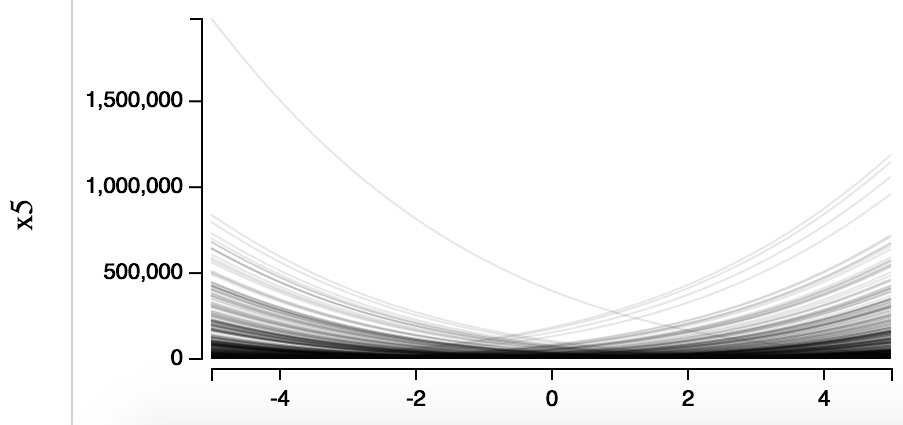
\includegraphics[width=\textwidth]{zakharov_confusing_unclustered.png}
    \caption{
    }
    \label{fig:cluster:none}
  \end{subfigure}
  ~
  \begin{subfigure}[b]{0.48\columnwidth}
    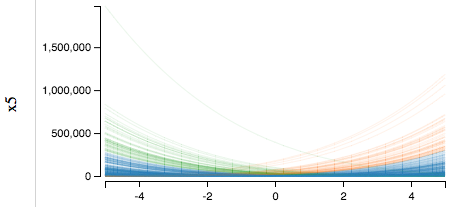
\includegraphics[width=\textwidth]{zakharov_color_clusters.png}
    \caption{
    }
    \label{fig:cluster:clustered}
  \end{subfigure}
  \caption[500 projected slices of the 5th dimension of the 5D Zakharov~\cite{Back:1996} function.]{%
    500 projected slices of the 5th dimension of the 5D Zakharov~\cite{Back:1996} 
    function. It is difficult to see if the slices are bowl shaped or two sets
    of monotonically decreasing and increasing curves. It is much clearer in 
    the cluster view that there are actually three sets of curves: 
    there is a set of monotonically decreasing curves and a set of 
    monotonically increasing curves. The very low-value curves form a third
    set.
  }
\end{figure}

Similar to visual encoding techniques such as parallel coordinate plots, projected 1D slices might mask certain patterns due to
overdrawing.
\autoref{fig:cluster:none} is an example where it is difficult to tell if the
slices are monotonic or bowl-shaped (\textbf{R-bowl}). The interactive slice highlighting
can give some insight into how individual slices are behaving but lacks
a global method to distinguish groups. Sliceplorer offers a
clustered slice view to address this (\autoref{fig:cluster:clustered}). 
The clustering is done with a k-nearest neighbor algorithm using the
$L^2$ distance between two slices as the distance metric.
This allows us to group the slices into distinct
groups of behavior and color-code these groups to distinguish them.

